\documentclass[12pt]{report}
\usepackage[a4paper]{geometry}
\usepackage[myheadings]{fullpage}
\usepackage{fancyhdr}
\usepackage{lastpage}
\usepackage{graphicx, wrapfig, subcaption, setspace, booktabs}
\usepackage[T1]{fontenc}
\usepackage[font=small, labelfont=bf]{caption}
\usepackage{fourier}
\usepackage[protrusion=true, expansion=true]{microtype}
\usepackage[english]{babel}
\usepackage{sectsty}
\usepackage{lipsum}
\usepackage{listings}
\usepackage{xcolor}
\usepackage{enumerate}
\usepackage{amssymb}
\usepackage{longtable}
\usepackage{courier}
\usepackage{geometry}
\usepackage{amsmath}
\usepackage{txfonts}
\usepackage{verbatim}
\usepackage{tikz}
\usepackage{adjustbox}
\usepackage{indentfirst}
\usepackage[colorlinks, linkcolor=blue, anchorcolor=blue, citecolor=blue, urlcolor=blue]{hyperref}

\usetikzlibrary{er,positioning,trees}
\newcommand{\HRule}[1]{\rule{\linewidth}{#1}}
\onehalfspacing
\setcounter{tocdepth}{5}
\setcounter{secnumdepth}{5}

\tikzset{every entity/.style={draw=orange, fill=orange!20}}
\tikzset{every attribute/.style={draw=purple, fill=purple!20}}
\tikzset{every relationship/.style={draw=green, fill=green!20}}

\lstdefinestyle{customc}{
  belowcaptionskip=1\baselineskip,
  breaklines=true,
  frame=shadowbox,
  rulesepcolor=\color{red!20!green!20!blue!20},
  numbers=left,
  numberstyle=\tiny,
  xleftmargin=\parindent,
  language=java,
  showstringspaces=false,
  basicstyle=\footnotesize\ttfamily,
  keywordstyle=\bfseries\color{blue},
  commentstyle=\itshape\color{gray},
  stringstyle=\color{red},
  xleftmargin=2em,
  xrightmargin=2em,
  aboveskip=1em
}

\lstdefinestyle{customjava}{ %
  language=Java,                  % the language of the code
  basicstyle=\footnotesize,       % the size of the fonts that are used for the code
  numbers=left,                   % where to put the line-numbers
  numberstyle=\tiny\color{gray},  % the style that is used for the line-numbers
  stepnumber=1,                   % the step between two line-numbers. If it's 1, each line
                                  % will be numbered
  numbersep=5pt,                  % how far the line-numbers are from the code
  backgroundcolor=\color{white},  % choose the background color. You must add \usepackage{color}
  showspaces=false,               % show spaces adding particular underscores
  showstringspaces=false,         % underline spaces within strings
  showtabs=false,                 % show tabs within strings adding particular underscores
  frame=single,                   % adds a frame around the code
  rulecolor=\color{black},        % if not set, the frame-color may be changed on line-breaks within not-black text (e.g. commens (green here))
  tabsize=4,                      % sets default tabsize to 2 spaces
  captionpos=b,                   % sets the caption-position to bottom
  breaklines=true,                % sets automatic line breaking
  breakatwhitespace=false,        % sets if automatic breaks should only happen at whitespace
  title=\lstname,                 % show the filename of files included with \lstinputlisting;
                                  % also try caption instead of title
  keywordstyle=\color{blue},          % keyword style
  commentstyle=\color{gray},       % comment style
  stringstyle=\color{purple},         % string literal style
  escapeinside={\%*}{*)},            % if you want to add a comment within your code
  morekeywords={*,...}               % if you want to add more keywords to the set
}

\lstset{style=customjava}

\makeatletter
\newcommand{\rmnum}[1]{\romannumeral #1}
\newcommand{\Rmnum}[1]{\expandafter\@slowromancap\romannumeral #1@}
\makeatother

\renewcommand{\labelenumii}{\theenumii}
\renewcommand{\theenumii}{\theenumi.\arabic{enumii}.}

\newcommand{\tabincell}[2]{\begin{tabular}{@{}#1@{}}#2\end{tabular}}

\renewcommand\thesection{\arabic{section}}

\pagestyle{fancy}
\fancyhf{}
\setlength\headheight{15pt}
\fancyfoot[C]{\thepage}

\setcounter{tocdepth}{2}


\begin{document}
\tikzstyle{table}=[draw=black,anchor=west]
%\tikzstyle{selected}=[draw=red,fill=red!30]
%\tikzstyle{optional}=[dashed,fill=gray!50]
\title{
        \HRule{2pt}\\
        \LARGE \textbf{\uppercase{Documentation of\\ Social Network Project}}
        \HRule{2pt} \\ [0.5cm]
        \normalsize \today \vspace*{5\baselineskip}}

\date{}

\author{He Yan}

\maketitle
\tableofcontents
\setcounter{page}{0}
\thispagestyle{empty}
\newpage

\section{Introduction}
%\addcontentsline{toc}{section}{Introduction}

This project aims to build a social network with JSP and MySQL.

\subsection{Main Features}
\begin{itemize}
	\item \emph{Compulsory}:
		\begin{itemize}
			\item Sign up \& in
			\item Search for contacts \& Post status and reply
			\item 30 secs refreshment
		\end{itemize}
	\item \emph{Optional}:
		\begin{itemize}
			\item Email address regex check
			\item Ajax
			\item Add Google's reCaptcha\footnote{Completely Automated Public Turing test to tell Computers and Humans Apart} validation
			\item Two-step friends
		\end{itemize}
\end{itemize}

\subsection{Components}
\begin{itemize}
	\item Apache, Tomcat, Apache-Tomcat-Connector
	\item MySQL, MySQL Connector/J (JDBC)
\end{itemize}

Visit our project site at \href{http://54.250.244.23/database-project/db/main.jsp}{Database Course Project}.

\section{Environment}

This project is hosted on Amazon Linux AMI server provided by AWS. To build the environment for running our website, we took steps as below.

\begin{enumerate}
	\item install OpenJDK-1.8.0
	\item install and configure Apache (httpd) \& Tomcat
	\item link Apache and Tomcat with Apache Tomcat Connector \footnote{This makes it possible to run static web pages on Apache and dynamic ones on Tomcat.}
	\item install MySQL\footnote{MySQL is case insensitive for Windows and MacOS, but that's not true for Linux.} and prepare MySQL connector/J in WEB-INF/lib
\end{enumerate}

Note: Our project has been hosted at GitHub. Visit our project at \url{https://github.com/PKU-2017-Database/Social-Network}.

\section{Data Structure}

\subsection{Entity-Relationship Diagram}

Here is an English version of ER Diagram redrawn by \LaTeX.

\begin{figure}[htbp]
	\begin{center}
		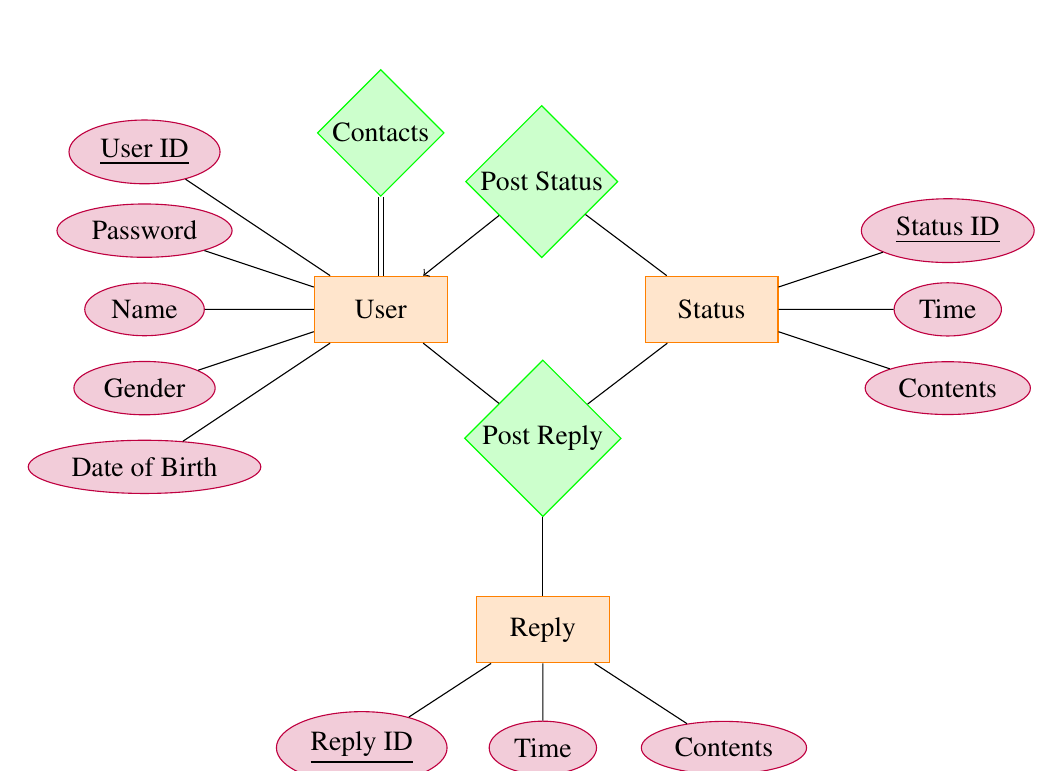
\begin{tikzpicture}[auto,node distance=1cm]
  % Create an entity with ID node1, label "Fancy Node 1".
  % Default for children (ie. attributes) is to be a tree "growing up"
  % and having a distance of 3cm.
  %
  % 2 of these attributes do so, the 3rd's positioning is overridden.
  \node[entity] (node1) {User}
    [grow=left,sibling distance=1cm, level distance=3cm]
    child {node[attribute] {\underline{User ID}}}
    child {node[attribute] {Password}}
    child {node[attribute] {Name}}
    child {node[attribute] {Gender}}
    child {node[attribute] {Date of Birth}};
    %child[grow=left,level distance=3cm] {node[attribute] {Attribute 3}};
  % Now place a relation (ID=rel1)
  \node[relationship] (rel1) [above = of node1] {Contacts};
  \path (rel1) edge [double distance=1.5pt] (node1);

  \node[relationship] (rel2) [above right = of node1] {Post Status};
  \node[relationship] (rel3) [below right = of node1] {Post Reply};

  \node[entity] (node3) [right = 2.5cm of node1] {Status}
    [grow=right, sibling distance=1cm, level distance=3cm]
    child {node[attribute] {Contents}}
    child {node[attribute] {Time}}
    child {node[attribute] {\underline{Status ID}}};


    \node[entity] (node2) [below = of rel3] {Reply}
      [sibling distance=2.3cm]
      child {node[attribute] {\underline{Reply ID}}}
      child {node[attribute] {Time}}
      child {node[attribute] {Contents}};

  \path (rel2) edge [->] (node1) edge (node3);
  \path (rel3) edge (node1) edge (node3) edge(node2);
  % Now the 2nd entity (ID=rel2)
  %\node[entity] (node2) [above right = of rel1]	{Fancy Node 2};
  % Draw an edge between rel1 and node1; rel1 and node2
  %\path (rel2) edge node {1-\(m\)} (node1)
   % edge	 node {\(n\)-\(m\)}	(node2);
\end{tikzpicture}

	\end{center}
	\caption{Entity-Relationship Diagram}
\end{figure}

\subsection{MySQL Table}

According to the above ER Diagram, we've designed MySQL tables as below.

\begin{figure}[htbp]
\begin{center}
\input{sqltb.tex}
\end{center}
\caption{MySQL Table Structure}
\end{figure}

Details about tables and attributes:

\input{tbdetail.tex}

\section{Division of Labor}

Our group members:

\begin{table}[htbp]
	\begin{center}
		\input{grpmem.tex}
	\end{center}
	\caption{Group Members}
\end{table}

Division of labor:

\begin{itemize}
	\item He Yan: write documentation \& add reCaptcha to website
	\item Sun Meng: design of website appearance
	\item Wu Chuchuan: logical framework \& database implementation
\end{itemize}

\section{Kernel Codes}

\subsection{Google reCaptcha}
\begin{lstlisting}
/* Client Side */
<div class="g-recaptcha" data-sitekey="6LdDNiMUAAAAAHDPfsdqqPKAPFEy5Xi3EoGwJIXi"></div>

/* Server Side */
String gRecaptchaResponse = request.getParameter("g-recaptcha-response");
String url = "https://www.google.com/recaptcha/api/siteverify";
String secret = "6LdDNiMUAAAAACVxX9eQOV4ITsc9YApSRpb80Lle";
boolean check = true;
if (!(gRecaptchaResponse == null || "".equals(gRecaptchaResponse))) {
	try{
		URL obj = new URL(url);
		HttpsURLConnection con =
			(HttpsURLConnection) obj.openConnection();
		con.setRequestMethod("POST");
		con.setDoOutput(true);

		String postParams
			= "secret=" + secret + "&response=" + gRecaptchaResponse;

		DataOutputStream wr =
			new DataOutputStream(con.getOutputStream());
		wr.writeBytes(postParams);
		wr.flush();
		wr.close();

		BufferedReader in =
			new BufferedReader(
				new InputStreamReader(
					con.getInputStream()));
		String inputLine;
		StringBuffer rsps = new StringBuffer();
		while ((inputLine = in.readLine()) != null) {
			rsps.append(inputLine);
		}
		in.close();

		JsonReader jsonReader =
			Json.createReader(
				new StringReader(rsps.toString()));
		JsonObject jsonObject = jsonReader.readObject();
		jsonReader.close();
		check=jsonObject.getBoolean("success");
	} catch(Exception e) {
		e.printStackTrace();
	}
}
...
if (check) {
	...
}
\end{lstlisting}


% TODO: add crucial codes of two-step friend
\subsection{Two-step friends}
% \begin{lstlisting}
\end{lstlisting}


% TODO: add image preview of website
\section{Website Preview}
% \includegraphics[width=100px,height=100px]{a.png}

\section{References}

\begin{itemize}
	\item Guidebook, installers and demo provided at \url{course.pku.edu.cn}
	\item \LaTeX \, template provided by \href{https://www.overleaf.com/latex/templates/project-template-titlepage/bwmhgfdvvhpw}{Overleaf}
	\item \href{https://dev.mysql.com/downloads/connector/j/}{mysql-connector-java-5.1.42-bin.jar}
	\item \href{https://mvnrepository.com/artifact/javax.json/javax.json-api/1.1}{javax.json-api-1.1.jar}
\end{itemize}

\end{document}
